
% Due Date: 7/23/14

\chapter{Relaxed Coherence}
\label{chapter:relaxed}
In this chapter we describe {\em relaxed coherence
modes} as an extension to the Legion programming 
model. Relaxed coherence modes improve both the 
expressivity of the programming model and enable 
higher performance for some Legion programs. The need
for relaxed coherence modes stems from a very
simple observation: not all programs require
direct data dependence ordering on access to 
logical regions. In many cases it is permissible
for tasks with interfering region requirements 
to be re-ordered as long as the runtime guarantees
a weaker property such as atomicity. Relaxed
coherence modes also allow applications to be more
precise regarding the kinds of properties that the
Legion runtime must guarantee when performing
dependence analysis between tasks. In this chapter
we discuss the introduction of two relaxed coherence
modes and their implementation in the Legion runtime.

\section{Relaxed Coherence Modes}
\label{sec:relaxedmodes}
By default, all region requirements specified in
a Legion program use {\em exclusive} coherence.
Exclusive coherence guarantees that at most one
task can be accessing the logical region named by 
a region requirement. Furthermore, exclusive
coherence ensures that interfering tasks are 
executed based on program order (the order in 
which they were issued to the runtime). This
guarantees that all data dependences are 
obeyed and program execution abides by serial
execution semantics. To allow programmers to 
relax the constraints describing how the Legion 
programming model handles tasks with interfering 
region requirements, we introduce two relaxed 
coherence modes: {\em atomic} and 
{\em simultaneous} coherence.

\subsection{Atomic Coherence}
\label{subsec:atomic}
Atomic coherence is a relaxed coherence mode that
allows Legion applications to specify that the 
accesses performed by a sub-task (or other operation)
on a logical region are required to be serializable
with respect to other operations. Serializability 
only ensures that interfering operations on the
same logical region are performed atomically with 
respect to each other, and not necessarily that they 
are performed in strict program order. This gives the
runtime the additional freedom to re-order tasks with 
interfering region requirements as long as both have 
requested atomic coherence. If either of the region 
requirements had requested exclusive coherence then 
re-ordering would not be sound as it would violate 
the semantics of exclusive coherence for one of the 
tasks. Atomic coherence is therefore useful for tasks 
that need to make atomic updates to a given region,
but permit re-orderings of operations with respect
to program order for higher performance. 

\subsection{Simultaneous Coherence}
\label{subec:simultaneous}
Simultaneous coherence is another relaxed coherence
mode that permits two tasks with interfering region
requirements to either be re-ordered or potentially
executed at the same time. The semantics of simultaneous
coherence allow re-ordering similarly to atomic coherence, 
making no guarantees about serializability. Instead,
simultaneous coherence permits two potentially 
interfering tasks to execute at the same time.
The one requirement on concurrent execution is that if
any interfering tasks are executing at the same time,
then they all need to immediately see updates from 
all the other executing tasks. For this to be
the case, the runtime must guarantee that simultaneously
running tasks that interfere on some region requirements
have been mapped to the same physical instance\footnote{
In the case of cache coherent memories, there is some
flexibility where the runtime can rely on the hardware
to maintain coherence.}, ensuring that updates are 
immediately visible to other interfering tasks. We describe 
the necessary changes to the physical region tree traversal 
for supporting the semantics of simultaneous coherence
in Section~\ref{subsec:physicalupdates}.

One important property of simultaneous coherence is that
it permits applications to effectively cut through some
of the standard Legion abstractions when programmers want
more control over expressing dependences (or lack thereof)
between different operations. Consequently, programmers
can express other programming paradigms without
the overhead and support of the Legion runtime. For example, an 
application may have stored a data structure such as a tree 
inside of a logical region. If the application attempts to 
launch many fine-grained tasks with atomic coherence to make 
modifications to the tree, it can result in considerable
runtime overhead. Instead, the application can launch
fewer tasks with simultaneous coherence on the region 
and rely on one of the finer-grained synchronization
primitives supported for simultaneous coherence that 
we discuss in Section~\ref{sec:syncprimitives}.

\subsection{Composability and Acquire/Release Operations}
\label{subsec:relaxedcompose}
Unlike privileges on logical regions that can be passed
from a parent task to a child task, relaxed coherence
modes apply only between sibling tasks. Consider, for
example, two sibling tasks $s_1$ and $s_2$ that both
request simultaneous coherence on the same logical 
region. If $s_1$ and $s_2$ execute in parallel,
then they can each launch child tasks with their own
coherence modes. Interference test are only performed
between tasks within the same context. It is the responsibility
of the application to handle synchronization between
tasks in different contexts accessing logical regions
with simultaneous coherence.

While it is the application's responsibility to manage
synchronization in these cases, it is the Legion 
runtime's responsibility to ensure the invariants of 
simultaneous coherence are met; specifically all updates
by a task (including all updates from its child tasks)
must be made visible in the simultaneous mapped region
immediately. In general, to provide the expected
behavior, child tasks of a task with a region using
simultaneous coherence must map to the same physical
instance to guarantee that updates are immediately
visible. Any region requirements for child-tasks
(or other operations) that derive their privileges
from a parent task region that was mapped with
simultaneous coherence is automatically marked by
the runtime as being {\em restricted}. This flag informs
the mapper that, regardless of any attempts to map the
task to a different physical instance, the runtime will
force the use of the same physical instance as the parent
task. This maintains two important invariants of the
Legion programming model: all updates for regions with
simultaneous coherence are immediately visible and
no mapping decisions can impact the correctness of
application execution. 

The restricted property provides for the enforcement
of simultaneous coherence semantics, but there are
many cases where application developers know that it
is safe to elide such restrictions. To communicate 
this information to the runtime, Legion provides an
explicit system of coarse grained software coherence
using {\em acquire} and {\em release} operations.
Issuing an acquire operation for a logical region that 
the parent task has mapped with simultaneous coherence
removes the restricted property, allowing sub-tasks
to map physical instances of the logical region in any 
potential memory. A corresponding release operation 
indicates that the restricted property should be enforced 
again. This invalidates all existing physical instances 
except the one initially mapped by the parent task and 
flushes all dirty data back to the originally mapped instance,
thereby making changes visible to other concurrent
tasks using the same physical instance. Like all 
operations in Legion, acquire and release operations
are issued asynchronously and the runtime automatically
determines the necessary dependences for actually
triggering execution of the operations. There are no
coherence annotations associated with acquire and 
release operations. Both kinds of operations behave
as if they were performed with exclusive coherence.

Unlike simultaneous coherence, atomic coherence does
not suffer from the same composability issues. Since
each parent task is guaranteed to have atomic access to
logical regions with atomic privileges, then all of
its child tasks can run and map in any possible memory.
Under these circumstances the naturally hierarchical
semantics of Legion task execution will flush any 
observable changes back to the mapped physical instance 
before the parent task completes and any of its
siblings can observe the changes.

\section{Synchronization Primitives}
\label{sec:syncprimitives}
When using simultaneous coherence with logical regions
it is the responsibility of the application to perform
any necessary synchronization in order to avoid data
races. There are two potential avenues for implementing
synchronization protocols in conjunction with simultaneous
coherence. First, users can implement their own
synchronization primitives and store them in logical regions
that are also accessed with simultaneous coherence. 
Simultaneous coherence guarantees that if two tasks are 
executing at the same time with privileges on interfering
logical regions, then they are using the same physical 
instance with reads and write being immediately visible.
Along with an atomic operation (e.g. compare-and-swap), 
this condition is sufficient to construct locks and similar
synchronization primitives. The alternative approach to
implementing synchronization in conjunction with simultaneous 
coherence is to use one of the two built-in synchronization
primitives provided by Legion: {\em reservations} 
(Section~\ref{subsec:reservations} and
{\em phase barriers} (Section~\ref{subsec:phasebarriers}).

\subsection{Reservations}
\label{subsec:reservations}
Reservations are the synchronization primitive provided 
by the Legion runtime for guaranteeing atomicity when 
accessing data in a region with simultaneous coherence.
Applications issue {\em requests} for reservations
that may or may not be immediately granted. If a task
with simultaneous coherence issues a request, then 
it must block and wait for the request to be granted
before continuing. Legion is able to preempt
a blocked task and schedule additional tasks until the
reservation is granted in order to hide the latency.
Alternatively, the task might issue child tasks and
request reservations on behalf of the child tasks.
Legion adds the reservation request as part of the 
prerequisites for the child task and ensures that 
the child task is not scheduled until the reservation
is granted. Reservations can be released at any point
after an acquisition.

Reservations support being acquired in different 
{\em modes} and with different {\em exclusivity} guarantees.
When a reservation request is made, the application
specifies the mode (e.g. an integer). A reservation
can be held in at most one mode at a time. Furthermore,
the exclusivity requirement states whether other users
are also permitted to hold the reservation in the given
mode at the same time. If exclusivity is requested,
then at most one user can hold the reservation at a
time. However, if exclusivity is not requested, 
then multiple users all requesting the same mode
(without exclusivity) are permitted to hold the
reservation at the same time. Exclusivity is useful
for supporting read-only cases where multiple users
of a given mode are acceptable because they are all
reading a data structure.

\subsection{Phase Barriers}
\label{subsec:phasebarriers}
The other synchronization primitive provided by the
Legion runtime for use with simultaneous coherence
are phase barriers. Phase barriers provide a way of
ordering access to logical regions in simultaneous
coherence. Unlike traditional barriers that block
waiting for all of the users of a resource to arrive,
phase barriers can be used to encode producer-consumer
relationships between subsets (or simply pairs) of
users. When phase barriers are created, the application
specifies the number of {\em arrivals} that must be 
observed before the {\em generation} of the barrier
advances. Arrivals are non-blocking operations performed
by tasks to signal that they have completed (produced)
some value and stored it in a logical region mapped with
simultaneous coherence. Similarly, other tasks can 
block waiting on a specific generation of a phase 
barrier. When a barrier advances to a new generation,
it triggers all the tasks waiting on the new generation,
indicating that it is safe to consume the results in a
logical region mapped with simultaneous coherence. It
is the responsibility of the application to maintain the 
association of phase barriers with simultaneously 
mapped logical regions.

Using phase barriers, applications can encode
producer-consumer relationships between tasks with
access to logical regions in simultaneous coherence.
This is especially useful for capturing common
communication patterns such as exchanging ghost cells
through logical regions with simultaneous coherence
as we will show in Chapter~\ref{chapter:s3d}. 

In order to use phase barriers safely, applications
need a crucial guarantee from the runtime regarding
the concurrent execution of tasks. Phase barriers 
require that all tasks participating in the synchronization
operation are executing at the same time to avoid
deadlock. In Section~\ref{sec:mustepochs} we discuss
the specific mechanism that Legion provides for 
applications to express this constraint of 
an application to the runtime.

\section{Must Parallelism Epochs}
\label{sec:mustepochs}
When developing programs with simultaneous coherence
and explicit synchronization between tasks, it is often
necessary for tasks to synchronize with each other
as part of their execution to make forward progress.
As an example, consider the S3D application described
in Chapter~\ref{chapter:s3d}. S3D creates explicit
regions for storing ghost cells and uses phase barriers
to synchronize between different tasks that have
mapped the explicit ghost cell logical regions with
simultaneous coherence. In order to avoid live-locking,
the application requires a mechanism for communicating
to the runtime that some tasks must be guaranteed to
be executing at the same time. Legion provides 
support for these cases with {\em must epochs}.

A must epoch is a collection of tasks that all must
execute concurrently on different processors, thereby 
making it possible for tasks to synchronize with each 
other. In some ways, this mirrors the semantics of 
traditional SPMD programming models such as MPI which
guarantee that all processes run concurrently and can
therefore synchronize with each other using barriers.
However, unlike traditional SPMD programming models,
the phase barriers and reservations available as 
synchronization primitives do not block the Legion
deferred execution model. Must epoch task launches
also differ in that they can be used at several 
different levels in the task tree. In practice, 
must epoch task launches are used infrequently
and mainly only when relaxed coherence modes are
necessary.

Must epoch task launches can consist of an arbitrary 
collection of individual and
index space task launches. The tasks that are launched
proceed through the standard dependence analysis 
independently, but the runtime captures the set of 
simultaneous coherence constraints that exist between
tasks within the must epoch launch. When all of the
tasks within a must epoch launch have had all their
mapping dependences satisfied, the runtime invokes
the {\tt map\_must\_epoch} call to map all of the
tasks within the must epoch. As part of the mapper
call, the runtime passes in all the simultaneous
coherence constraints that must be satisfied 
(e.g. region requirements that must all be mapped
to the same physical instance) in order for the
must epoch to be successfully mapped. The mapper then 
performs the equivalent of the {\tt map\_task}
mapper call for each of the tasks. It is the
responsibility of the mapper to satisfy all of
the mapping constraints or else the mapping
will fail. The mapper is also responsible for 
assigning each task in the must epoch to a different
target processor so that all the tasks can
execute concurrently. The runtime uses the results
of the {\tt map\_must\_epoch} call to perform
the mapping for each of the tasks. If all the
tasks successfully map, all the tasks are assigned
to different processors, and all the simultaneous
coherence constraints are satisfied, then the
must epoch mapping will be executed.

% Relation to SPMD and Pipeline parallelism
The introduction of must epoch launches has an 
interesting consequence for the design of the 
Legion programming model. Must epoch launches
allow applications to be written in a way that
permits longer running tasks that operate in 
parallel, communicating data through regions with
simultaneous coherence and synchronizing with
reservations or phase barriers. This property
makes it possible to write applications that
behave similarly to the SPMD applications 
discussed in Section~\ref{sec:programming}. The
primary difference being that Legion tasks 
written in this style are still executing in
a deferred execution model that confers considerably
more latency hiding ability that existing
SPMD approaches.

Long running tasks using regions mapped with
simultaneous coherence can also be used to 
implement applications that require pipeline
parallelism (e.g. \cite{GRAMPS09}), with 
different long running tasks performing the 
operation of different pipeline stages and 
logical regions mapped with simultaneous 
coherence storing queues of data. Must 
epochs give Legion the power to capture 
these patterns and thereby increase the 
expressivity of the programming model.

\subsection{A Complete Example}
\label{sec:completeex}
Initially all of the various features of relaxed
coherence modes may seem disparate and unrelated.
However, for many applications, all of the different
components are essential for using relaxed coherence
modes to achieve high performance. As a minimal 
example of how all these features compose, we 
introduce a very simple stencil example.

Consider a simple one dimensional stencil computed
using explicit ghost cell regions. In this scenario,
many parallel tasks are launched, each of which
requests privileges on the logical region of local
cells that it owns ({\tt local\_lr}), two logical 
regions of explicit ghost cells that it owns (
{\tt left\_lr} and {\tt right\_lr}), and the 
left and right ghost cell regions from its right
and left neighbor respectively. The region {\tt local\_lr}
is requested  with exclusive coherence, but the 
other regions are requested with simultaneous coherence
to enable all the tasks to run at the same time.
In order to permit the tasks to synchronize using
phase barriers, the tasks are all launched as part
of the same must epoch. Since they are all launched
in the same must epoch, the launching node
maps them all at the same time. Each task is assigned
a different processor and maps its {\tt local\_lr}
and neighbor {\tt left\_lr} and {\tt right\_lr} into
memories local to the target processor. The idea behind
this mapping is that tasks will push their data to 
the explicit copies of their owned {\tt left\_lr} 
and {\tt right\_lr} on remote nodes.

Figure~\ref{fig:stencilex} illustrates the execution of 
the stencil tasks for several iterations. When the tasks run, 
they may perform other computations on {\tt local\_lr}, but 
eventually they need to perform the stencil computation. To 
perform the stencil computation they first issue explicit
copies from their {\tt local\_lr} logical region to the 
ghost cell regions they own (which have been mapped into
memories on remote nodes). Phase barriers are triggered
contingent upon the completion of the copies to mark when
the data in the owned logical regions are valid. After
issuing the explicit copies, the tasks then perform an 
acquire request for the neighbor explicit ghost cell
regions contingent on the phase barriers from each
of their neighbors have triggered. The acquire operation
is necessary to gain coherence for the explicit ghost
cell logical regions so they can be moved if necessary.
In the specific case of Figure~\ref{fig:stencilex}, 
the acquire operation is necessary so the stencil 
computations themselves can be run on a GPU. After the
acquire operation is issued, the explicit stencil 
computation is launched (Legion automatically computes
the dependence based on region usage). After the 
stencil is performed, then a release operation is
issued to invalidate any copies of the explicit ghost
cell regions that were created. A second phase barrier
is triggered upon completion of the release operation 
to indicate that the results in the explicit ghost cell
regions have been consumed. Each of these phase barrier
triggers become a precondition for the next explicit copy 
request that is performed into the explicit ghost cell
regions to prevent write-after-read races.

\begin{figure}
\centering
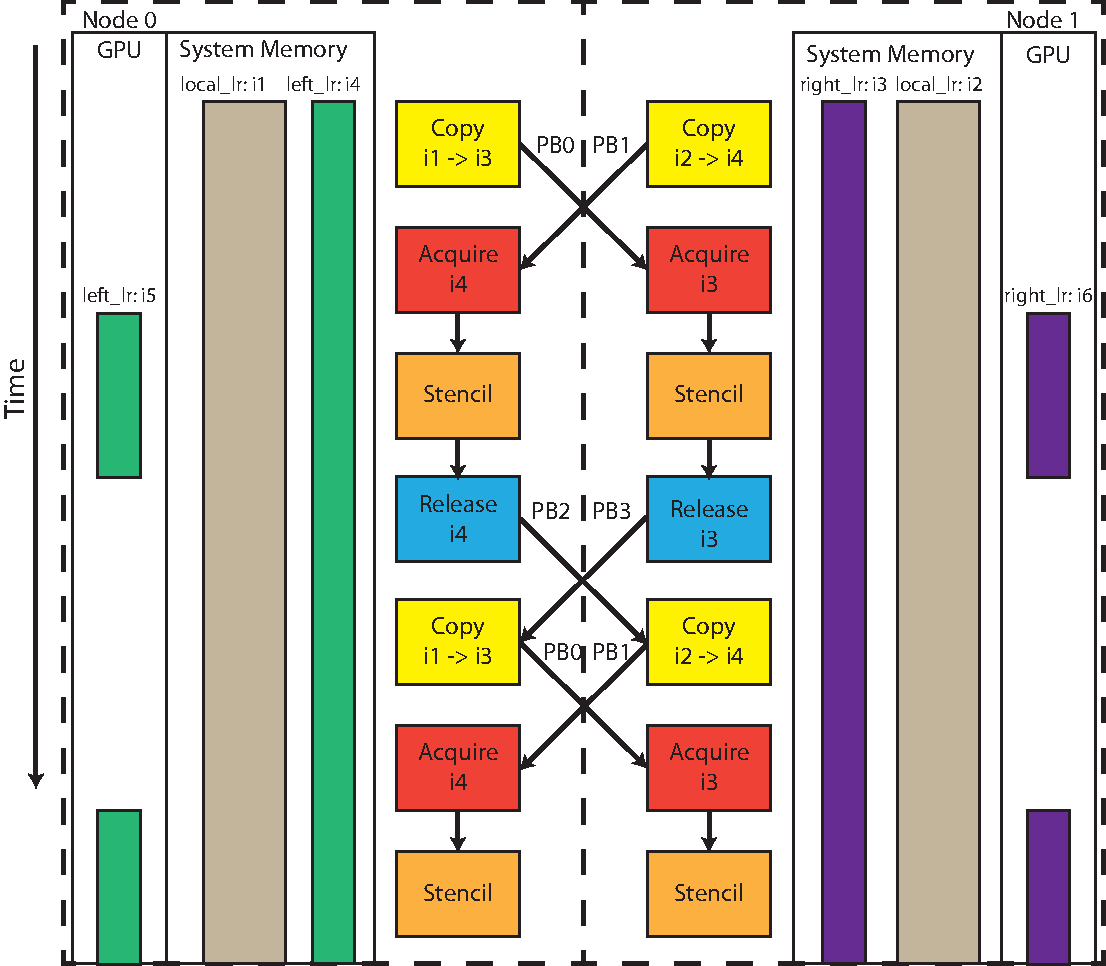
\includegraphics[scale=0.70]{figs/PhaseBarrier.pdf}
\caption{Example Use of Simultaneous Coherence and Related Features\label{fig:stencilex}}
\end{figure}

Figure~\ref{fig:stencilex} has three important properties.
First, once this stencil pattern of communication is
set up, tasks can run for arbitrarily long\footnote{Until
the phase barriers exhaust their $2^{31}$ generations.},
re-using the phase barriers over and over again. While
the pattern expressed here is sometimes difficult for 
human programmers to set up, it is trivial to generate
either as part of a library and or a higher-level 
language that targets Legion. 

The second interesting
property of this example is that the operations 
necessary for computing the stencil never block, 
thereby enabling continued deferred execution of
the tasks. This is especially important if the tasks
have significant additional work to do on {\tt local\_lr}
which is mostly non-interfering with the stencil 
computation (this will be the case with S3D as we
will see in Chapter~\ref{chapter:s3d}). The non-blocking
nature of the operations, even with their composition
with phase barriers, allows Legion to find additional
work to do while the long latency copy operations are
being performed.

Third, while the pattern set-up in this example is
relatively simple, more complex double- and triple-buffered
algorithms can be employed for further latency hiding.
The choice of the buffering depth is often application
and machine dependent and it is easy to parametrize
the buffering depth as a tunable variable that can be
changed by the mapper. Legion applications therefore
have a rich set of possibilities available to them 
for exchanging data between executing tasks using 
explicit logical regions.

This stencil example shows how all the different
components associated with relaxed coherence modes
compose naturally and can be used to write high 
performance distributed code. In practice, all of
these features will be used as part of our implementation
of the S3D combustion simulation in Chapter~\ref{chapter:s3d}.


\section{Tree Traversal Updates}
\label{sec:relaxedupdates}
In order to support relaxed coherence modes,
several changes need to be made to both the
logical and physical region tree traversal
algorithms from Chapters~\ref{chapter:logical}
and \ref{chapter:physical}. In this section
we describe the general modifications to both
the traversal algorithms as well as the
additional state added to the region tree 
data structures for supporting these 
additional traversals.

\subsection{Logical Tree Updates}
\label{subsec:logicalupdates}
There are several modifications that need to
be made to the logical region tree traversal
algorithm. First, there is a slight modification
to the definition of interference for relaxed
coherence modes. While both atomic and 
simultaneous coherence modes prevent interference
on region requirements that would normally be
interfering if exclusive coherence was used,
for the logical traversal it is still important
to detect any potential interference and register a
mapping dependence. The reason is that relaxed
coherence modes only prevent non-interference
if the two region requirements are ultimately
mapped to the same physical instance. If they
fail to map to the same physical instance, then
the runtime will need to inject a copy to move
the data that will ultimately serialize the
execution of the two tasks and elide the need
for relaxed coherence. In order to detect whether 
the two potentially interfering region requirements
both map to the same physical instance or not, 
the mapping of the two different region requirements 
therefore must be serialized by a mapping dependence.

To detect these additional mapping dependences
the majority of the region tree traversal remains
the same.  Traditional tests for non-interference
based on logical regions, fields, and privileges
all remain the same. However, for cases where 
non-interference would normally be detected based
on relaxed coherence modes, mapping dependences are
recorded. It is possible that these mapping dependences
ultimately will not result in any event dependences
in the event graph, but the result depends on the
chosen mapping. While these additional mapping
dependences for relaxed coherence modes do serialize
some aspects of the region tree traversal, in 
practice we have found the latency hiding capabilities
of Legion's deferred execution model to be 
sufficient for eliminating any additional overhead.

The second modification that must be made to the
logical region tree traversal algorithm is the 
addition for tracking whether mapping of any region
requirements are restricted because an ancestor
task initially mapped a region with simultaneous
coherence. The initial part of detecting mapping
restrictions is done before traversal begins. 
Each parent task records which of its physical
instances were restricted when it mapped. If the
parent task was either restricted or directly 
requested simultaneous coherence, then any child
tasks with region requirements that subsume their
privileges from the restricted region must also
be restricted. If either of these cases hold, then
the appropriate region requirements of the child
task are also marked restricted.

After a child task has completed its logical 
dependence analysis for a region requirement, it
then checks to see if the chosen requirement is
also potentially restricted. If the requirement
is restricted due to simultaneous coherence, then an
additional traversal is necessary to detect
whether there are any outstanding acquire
operations that might remove the restriction.
To support detecting such cases, we first 
annotate each node on the logical region tree
with a field mask for storing which fields
for that particular logical region have 
acquired user-level coherence. When an 
acquire performs its logical dependence analysis, 
it records no dependences\footnote{The acquire operation
does not need to record any mapping dependences
as it simply modifies the state of the logical
region tree.}, but instead mutates 
all the fields in the user level coherence mask 
in the logical node for which user-level coherence 
was requested. The acquire operation then recurses
down all sub-trees from the acquired logical region
annotating all user-level coherence field masks
as well. Release operations have the 
opposite effect of unsetting the flags in the
user-level coherence bit masks as later operations.
Unlike acquire operations, release operations 
undergo the standard mapping dependence traversal
for its region requirement as it will be required
to actually perform operations on the physical
region tree as we will discuss in 
Section~\ref{subsec:physicalupdates}.

Using the user-level coherence bits, operations
that might otherwise be restricted can detect
if they actually have acquired user-level coherence
and can therefore avoid any mapping restrictions.
After an operation completes its normal logical
dependence analysis traversal for a region 
requirement, if the region requirement 
is possibly restricted based on analysis of its
parent task's regions, then the operation can 
traverse the path from where the parent task
has privileges to where the region requirement
is requesting privileges to detect if
user-level coherence has been acquired on 
any of the logical regions. If all of the fields
for the region requirement can be shown to 
be in an acquired state, then the restriction
on mapping due to simultaneous coherence can
be removed.

\subsection{Physical Tree Updates}
\label{subsec:physicalupdates}
There are fewer modifications to the physical
dependence analysis than for the logical 
dependence analysis. The most obvious change
involves region requirements that are restricted
due to simultaneous coherence. In these cases,
any input from the mapper is ignored and the 
runtime proceeds to use the physical region 
mapped by the parent task. If the physical region
is not visible from the target processor then 
the mapping will fail and the runtime reports 
that an invalid target processor was selected.

The next modification that is made is for
supporting the instance view traversal algorithm.
In this case, the interference test for users
is modified such that interference between two
users both requesting atomic coherence, or two
users both requesting simultaneous coherence
is elided so that no interference results. Recall
that an instance view only stores data for users
of the same physical instance; therefore two
users testing for interference within the same
instance view have already satisfied the constraint
for relaxed coherence modes that they use
the same physical instance. If two tasks with a
mapping dependence based on relaxed coherence modes
map to different physical instances, then the copy
generated by the Legion runtime is sufficient to 
properly serialize the execution of the two tasks.

In the case where the two tasks both request 
atomic coherence, the runtime uses the low-level
runtime reservations to mediate atomic access to 
the physical instance. Due to the large number of
fields associated with many physical instances,
the runtime uses a few reservations per physical
instance and maps different fields onto 
different reservations. While
this may in some cases result in unnecessary
synchronization between tasks, in general it
is not problematic and is better than maintaining
a single reservation used for each physical 
instance which could lead to considerable 
unnecessary synchronization.

\section{Implications for Hardware}
\label{sec:hardimpl}
Relaxed coherence has many potential implications
for the design of hardware systems for both 
performance and power efficiency. In this section,
we discuss how two different kinds of hardware
improvements could be automatically employed by
Legion and the potential benefits for hardware.

\subsection{Transactional Memory}
\label{subsec:tm}
Currently, the implementation of atomic coherence
in Legion is based on the software-level reservation
primitive provided by the low-level runtime. This
leads to a very coarse-grained approach to synchronizing
access to physical instances. Another approach would be
the use of either a hardware or hybrid transactional memory 
system to allow multiple tasks to execute concurrently 
using the same physical instance. If conflicts between
the tasks resulted in an execution that was not 
serializable the transactional memory could automatically
abort the affected tasks and restart them. This could
considerably improve the throughput of tasks that use
atomic coherence and would also remove any potential
for false serialization resulting from the shared
reservation scheme described in 
Section~\ref{subsec:physicalupdates}.

\subsection{Hardware Coherence}
\label{subsec:hwcoher}
Another potential improvement afforded by relaxed 
coherence modes is the ability to elide hardware coherence
for large ranges of virtual memory. Legion coherence
modes are precise enough to know exactly which memory
allocations need support from the hardware for providing
cache coherence.  Specifically, only physical instances
using simultaneous coherence and internal runtime data
structures would require hardware cache coherence. For
all other physical instances (which for most applications
is the majority of memory) hardware cache coherence 
could be disabled. The large power cost of hardware 
cache coherence could be considerably lessened, allowing
for more efficient hardware. Furthermore, giving a programming
system like Legion the ability to manage hardware caches
using software primitives could ultimately lead to higher
performance by explicitly mapping different logical 
regions into different caches for specific tasks, resulting
in higher performance and lower power due to less data
movement.

